\section{Clock Generator}

The clock generator derives an ultra-low-jitter timing reference from the single-ended \SI{10}{\mega\hertz} backplane synchronization signal (\texttt{CLOCK\_SYNC}). We use the Skyworks Si5342A-D jitter-attenuating clock multiplier, which provides:

\begin{itemize}
    \item Ultralow \SI{90}{\femto\second} RMS output jitter.
    \item Support for external crystals between \SI{25}{\mega\hertz} and \SI{54}{\mega\hertz}.
    \item SPI/I²C control interface.
    \item Zero-delay mode for minimal, deterministic input-to-output latency.
    \item Both single-ended and differential I/O.
\end{itemize}

The Si5342A-D “cleans” the backplane clock to produce a low-jitter reference. The Zynq SoC then employs this cleaned clock for its sequencer timing and to drive the DC-DC converters, reducing their switching noise and improving overall power-rail integrity.

In our design (see \autoref{fig:clock_gen}), a Kyocera AVX \SI{48}{\mega\hertz} $\pm$ 10ppm crystal provides the Si5342A-D's reference frequency. The device is configured in zero-delay mode to guarantee a fixed, repeatable phase relationship between \texttt{CLOCK\_SYNC} and the output clock to Zynq SoC. Configuration and status monitoring are handled over I²C via the Zynq SoC's. Finally, the Si5342A-D's differential \SI{2.5}{\volt} LVDS output is routed directly into one of the Zynq SoC's MRCC (Multi-Region Clock-Capable) input.

\begin{figure}[ht]
  \centering
  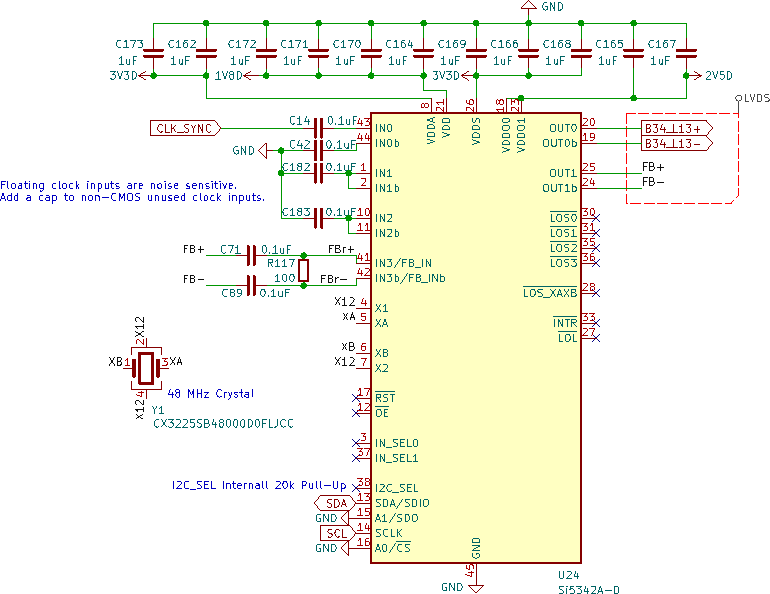
\includegraphics[width=0.8\linewidth]{sections/clock_gen/fig_clock_gen.pdf}
  \caption{Si5342A-D Clock Generator Jitter Attenuator Circuit}
  \label{fig:clock_gen}
\end{figure}